%%%%%%%%%%%%%%%%%%%%%%%%%%%%%%%%%%%%%%%%%%%%%
% Template for Master and Bachelor theses   %
% at DSV, an adaptation made by Beatrice    %
% Åkerblom of the                           %
%%%%%%%%%%%%%%%%%%%%%%%%%%%%%%%%%%%%%%%%%%%%%
% Template for Doctoral Theses at Stockholm %
% University. The template is based on      %
% the layout an typography used in for      %
% dissertations in the Acta Univeristatis   %
% Upsaliensis series                        %
% Ver 3.0 SU - 2006-09-28                   %
%                                           %
% Erik Siira                                %
% erik.siira@ub.uu.se                       %
% Tel. 471 39 70                            %
%                                           %
% Special thanks to                         %
% Anders Källström,                         %
% Robert Nyqvist                            %
% and other studens who have used the       %
% former version of this template and       %
% submitted valuable feedback.              %
%%%%%%%%%%%%%%%%%%%%%%%%%%%%%%%%%%%%%%%%%%%%%


\documentclass[12pt,
               a4,
%               swedish,     % Uncomment this line if you write in Swedish
               twoside,
               openright]{book} % Default font 11pt, all pages are
                                % printed the same, new chapter always
                                % begins on a right-hand page.

% \usepackage[frame,a4,center]{crop} % Mount on A4 paper for preview
%% Use this (by uncommenting) if your printer complains that the paper
%% size is not A4.  Don't use it when the final version is produced.


% Package import
% Language, diacritics and hyphanation
               \usepackage[swedish,english]{babel} % Use English
                                                   % and Swedish
                                                   % languages. English
                                                   % default. English
                                                   % hyphenation.
               % \usepackage[latin1]{inputenc} % Unix users should
                                             % include this
                                             % package instead of
                                             % ansinew or applemac
                                             % for correct
                                             % handling of
                                             % diacritics.
              % \usepackage[applemac]{inputenc} % Macintosh users
                                                % should include this package 
                                                %instead of ansinew or latin1 
                                                %for correct handling of diacritics.
              %\usepackage[ansinew]{inputenc}  % Windows users include this package 
                                               %instead of applemac or latin1 for 
                                                %correct handling of diacritics. 
              \usepackage[utf8]{inputenc}
              % \usepackage{hyphenat}
\usepackage[T1]{fontenc}

% Page elements
\usepackage{mathptmx} % Default font for dissertations is Times.
%\usepackage{fourier} % If mathematics don't display well using
                      % Times, then use Fourier.
\usepackage{helvet}  

\usepackage{ThesisSU} % This package is specific for theses
                      % written at Stockholm University. 
                      % Modifications to the classfile and the 
                      % document can be found here.
%\ifpdf
%   \usepackage[pdftex]{graphicx}
%  \else
%    \usepackage[dvips]{graphicx}
%\fi % Used for figures

% need to use dvipdfm (current build order latex->bibtex->latex->latex->dvipdfm)
\usepackage{graphicx}
\graphicspath{{Figures/}}
\DeclareGraphicsExtensions{.eps}

% trying instead of below
 \usepackage{url}

%\usepackage[backref, colorlinks=true, urlcolor=black, pagecolor=black,
%linkcolor=black, citecolor=black, filecolor=black,
%menucolor=black, pdfpagelayout=TwoColumnRight, pdfstartview=FitH,
%plainpages=false,
%pdfpagelabels]{hyperref} % Use this package to obtain links in the
                         % electronic version of the document. All
                         % hyperlinks and other links
                         % should be black. Page view is set to
                         % Fit Width and page layout is set to
                         % display the document spread.  Make page
                         % anchors using the formatted form of the
                         % page number.  Set PDF page labels;
                         % i.e., write the value of \thepage to
                         % the PDF file so that Acrobat Reader can
                         % display the page number as (say) 'ii (4
                         % of 40)' rather than simply '4 of 40'.
                         
\usepackage{enumitem}
\setdescription{font=\normalfont\textit}

% Bibliographic information
% Filling in this bibliographic information facilitates the
% processing of this document.

% Insert linebreaks if necessary

% Just leave the posistion blank for any information that doesn't
% apply for your thesis, e.g. if your thesis doesn't have a subtitle:
%
% \newcommand{\thesisSubtitle}{}




% Abstract and titelpage

\firstAuthorFirstName{Thomas}                % First author given name
\firstAuthorSurname{Speckert}                 % First author surname
\secondAuthorFirstName{}              % Second author given name
\secondAuthorSurname{}                % Second author given name

\firstAuthorEmail{thsp7525@student.su.se}              % First author's e-mail address
\secondAuthorEmail{}             % Second author's e-mail address

\thesisTitle{Enterprise Architecture for Decentralized Environments}                   % The title of the thesis
\thesisSubtitle{} % The subtitle of the thesis 

\thesisSubject{Computer and Systems Sciences}   % May be changed
                                                % to e.g. Human-Computer 
                                                % Interaction or other 
                                                % suitable for your thesis 
\thesisIsKind{Master}                           % Change to Bachelor if suitable
\theYear{2013}
\thesisCred{30}                                 % Change to 15 if Bachelor
\thesisAdvisor{Jelena Zdravkovic}
\thesisAssistantAdvisor{}                       % Name of Assistant Advisor,
                                                % if you have one
\thesisExternalAdvisor{Irina Rychkova}                        % Name of External Advisor,
                                                % if you have one

\thesisReviewer{Name of Reviewer}
\semester{Spring}
\swedishTitle{Företagsarkitektur för Decentraliserade Miljöer}

                                               % The abstract text comes
                                               % here. Not more than 300
                                               % words. No empty lines.                                     
\abstracttext{ Qui terempri isuam liam incum aris forteat
  strudentre quid inculoc iviliaet; nihilius. Catimor demquam tam,
  senterf rmactum ompec orum, ne culvitimis se constusquam
  pratastiam porum rem, que poptert batia vidiem, sendum patus?
  Paturo vis esum inessus, furnimi iliciem ent vidit rebaturei
  potiu quam ductame teris, conductam me consum retis consuniu ma,
  speriam rem firisum publi, quam factod norehem et grat. Maesse,
  se orteliciemus cem.  Fuidena ilicien ervid C. M. C. me quid rem
  moente, conimus nit practanti, tabena, Ti. Habunterfer que
  avoltum quam hinaterniam abem nonside labistiae, intelic vidi
  ium erce enatici ecturox nulviribem hostio nesimoeritia rei
  inatis.}

\keywords{enterprise architecture, distributed computing, decentralized organizations}




 % This file should be edited by the author.

\begin{document}
  
    \frontmatterDSV % Sets the frontmatter (Title page(s), abstract, keywords, etc.)
    
    \tableofcontents
    
    % Optional tables
    %\listoftables
    %\listoffigures
    \chapter{Introduction}
    \label{chap:introduction}
    % Include your chapters here.
    
    \section{Background}
    \label{sec:background}
    \section{Background}
This is my background

    \section{Problem}
    \label{sec:problem}    
    \chapter{Problem}
Classical frameworks and methods for enterprise architecture are typically geared towards more centralized environments. As organizations trend towards decentralization, a need for a decentralized EA becomes apparent.
    
    \section{Research Questions}
    \label{sec:resq}
    \chapter{ResearchQuestions}
The project will seek answers to the following research questions:
\begin{enumerate}
\item In the scope of this project, what is meant by decentralization?
\item What is the definition of enterprise architecture?
\item What are the current major methods and frameworks for enterprise architecture?
\item What is the current state of decentralized enterprise architectures?
\item Are current enterprise architecture concepts and frameworks suitable for application in decentralized environments?
\item Can current knowledge decentralization be used to enhance our understanding of enterprise architecture?
\end{enumerate}
    
    % Part 2, Scientific Base
    
    \chapter{Extended Background}
    \label{chap:extendedBackgrounf}
    
    \section{Enterprise Architecture}
    \label{sec:ea}
    % The thesis should have an introduction to the research area to which the thesis belongs. The thesis should have the author’s own discussion about previous solutions to the problem that is being addressed. The thesis should also have the author’s own discussion about which scientific articles that the thesis builds upon and a motivation as to why these were chosen. Relevant theories should be discussed for the problem and research question, but or a Bachelor’s thesis it is not necessary that it is based on such theories.

% Requirement for 1 point: that the thesis provides a base for the topic of the thesis based on previous scientific research. The area within computer and system sciences to which the thesis contributes should also be named by presenting the scientific research to which the thesis refers. 

% For 2 points the following is also required: that a deep and critical discussion is made about how the thesis builds upon previous scientific research. 

% For 3 points the following is also required: that a systematic and comprehensive literature study is presented that is the basis for placing and evaluating the research contribution of the thesis in a scientific context.


\subsection{Overview}
According to Sessions~\cite{sessions2007}, the field of Enterprise Architecture (EA) emerged in order to combat two increasingly prevalent problems facing enterprises: system complexity and business-IT alignment. As enterprises rely more and more on information systems of increasing complexity, these problems become even more important. The field of EA views the solution to these problems to be one of concurrent design. It is not enough simply try and fit IT to the business; business and IT aspects should be designed concurrently. 

While there is no singular agreed-upon definition for EA, different definitions\cite{jungle2004,GartnerInc,ross2006,pearlson2009,lankhorst2009,sessions2007,togaf9.1} do have much in common. EA is a discipline that takes a holistic approach to transforming high-level business vision and goals into the integration of an enterprise's organizational structure, business processes, and information systems. This transformation involves identifying and implementing the necessary change for this to occur. The various EA frameworks aim to accomplish this through some or all of the following three phases [ACTUALLY THIS IS HOW WE ARE ANALYZING THEM, NOT NECESSARILY HOW THEY ARE ORGANIZED]: the preliminary phase, the EA description phase, and the EA engine phase. 

The preliminary phase aims to lay the groundwork for the EA process. Typically, this involves setting up teams, ownership, responsibilities and gaining commitment. The EA description phase is involved with creating the actual architecture artifacts (eg. models, principles) themselves. This generally involves outlining an enterprises EA principles, its as-is EA description,  the planned to-be architecture, an analysis of the gap between the as-is and to-be architectures and a plan to cross that gap. The engine  phase involves setting up a support structure for ensuring the ongoing adoption of the to-be EA description. This can involve gaining commitment from stakeholders, setting up some compliance checking procedures, and deciding upon a prioritization of tasks to be completed. The remainder of this section will look at 4 [NEED THE REAL NUMBER HERE] different EA frameworks from the perspective of of these three phases. 

[Requirements Management? - maybe 3rd phase]

% *Definition*
% 
% (1) http://www.gartner.com/it-glossary/enterprise-architecture-ea/
% Enterprise architecture (EA) is a discipline for proactively and holistically leading enterprise responses to disruptive forces by identifying and analyzing the execution of change toward desired business vision and outcomes. EA delivers value by presenting business and IT leaders with signature-ready recommendations for adjusting policies and projects to achieve target business outcomes that capitalize on relevant business disruptions. EA is used to steer decision making toward the evolution of the future state architecture.
% 
% (2) Nameless Book from Jelena
% Enterprise architecture (EA) is the process of translating business vision and strategy into effective enterprise change by creating, communicating and improving the key requirements, principles and models that describe the enterprise's future state and enable its evolution.
% 
% (3) MIT Center for Information Systems Research (MIT CISR) [but from Jelena's book]
% Enterprise architecture is the organizing logic for business processes and IT infrastructure reflecting the integration and standardization requirements of the company's operating model. The operating model is the desired state of business process integration and business process standardization for delivering goods and services to customers.

% (4) TOGAF
% The purpose of enterprise architecture is to optimize across the enterprise the often fragmented legacy of processes (both manual and automated) into an integrated environment that is responsive to change and supportive of the delivery of the business strategy.
% 
% (5)~\cite{lankhorst2009}
% a coherent whole of principles, methods and models that are used in the design and realisation of an enterprise's organisational structure, business processes, information systems, and infrastructure

% (6) 
% Op't Land, M.; Proper, E.; Waage, M.; Cloo, J.; Steghuis, C. (2009): Enterprise Architecture: Creating Value by Informed Governance. 1 ed. Springer, Berlin.
% “a continuous process involving the creation, modification, enforcement, application, and dissemination of different results. This process should be in sync with developments in the environment of the enterprise as well as developments internal to the enterprise, including both its strategy and its operational processes” [18].

\subsection{The Open Group Architecture Framework (TOGAF)}
The Open Group Architecture Framework, more commonly know as TOGAF, is a freely available EA framework created by The Open Group~\cite{togaf9.1}, a consortium of IT organizations. [SOMETHING ABOUT WHETHER A CONSORTIUM OF IT COMPANIES IS GOOD FOR INNOVATION, PERHAPS MORE FOR STANDARDS --> by corporations, so meant for corporate world]. 

TOGAF is comprised of a number of different aspects, mainly: the Architecture Development Method (ADM), "a method for developing and managing the lifecycle of an enterprise
architecture"~cite{togaf9.1}; the Architecture Content Framework, the companion to the ADM which describes the content of the products of the ADM; and the Enterprise Continuum, which provides a means to organize the produced architectures. 

[SOMETHING ABOUT FLEXIBILITY AND ITERATION]

3 levels of iteration:
- multiple ADMs to create different architectures
- within ADM
- change

ADM, Continuum,  \cite{lankhorst2009}

\subsubsection{Preliminary Phase}
TOGAF has a very well defined preliminary phase. TOGAF lays the groundwork for the rest of the EA process in the first two phases of the ADM: the Preliminary phase [CONFUSING, SAME NAME?] and the Architectural Vision phase. In TOGAFs preliminary phase, the primary tasks are to:
\begin{enumerate}
% \item Identify affected parts of the enterprise
\item Have the stakeholders agree on the expected effects of the TOGAF process
\item Set an architecture governance structure
\item Set up and gain approval for the EA team 
\item Outline the overarching architecture principles for the enterprise and ensure corporate management supports them (Perlim and A)
\item Tailor TOGAF to fit the enterprise
\item Create a repository for storing all architectural information and populate it with any already existing relevant artefacts relating to the current state of the enterprise
\end{enumerate}
~cite{togaf9.1}

The Architectural Vision phase includes the following tasks:
\begin{enumerate}
% \item Identify all relevant stakeholders
\item Establish architecture project
% \item Readiness
\item Elicit the management-approved business goals, requirements and constraints and use them to create a high-level vision for the enterprise's target and baseline architectures. 
\item Identify architecture acceptance criteria (e.g. milestones or metrics)
\item Create an architecture project plan and schedule
\end{enumerate}

Take the above and organize into a Statement of Architecture Work to be approved by the project sponsors and may form the basis of a contract between the architecture provider and the client. 

- more about stuff relating to problems


\subsubsection{Architecture Definition}
TOGAF views architecture from the perspective of four different architecture domains~\cite{sessions2007}: business, application, data, and technical. Business architecture is concerned with processes and functions used to meet business goals, application architecture is concerned with the design of specific applications and their interactions, data architecture is concerned with managing enterprise data, and the technical architecture is concerned with the infrastructure (hardware and software) used to support the applications. The architectures in these four domains are created through the ADM phases B (Business Architecture Phase), C (Information Systems Architectures Phase) and D (Technology Architecture).

- Multiple iterations throughout BCD to accomplish the Architecture Development

- Multiple iterations focusing on EF for Transition Planning

- Baseline or Target-first approach. Baseline for "decentralized"/"This approach is common where organizational units have had a high degree of autonomy."

- Similar process:
    - Select relevant viewpoints and appropriate models to best represent stakeholders. Important to ensure that all stakeholder concerns are covered
    - 


- definition of what's in a TOGAF architecture (Content Framework, Continuum)

- ADM phases B,C,D, EF (Roadmap/Migration Plan)

ROADMAP
- Work packages
- Gap Analysis results
- Transition Architectures

MIGRATION PLAN
- Groups the work packages into projects and schedules them

The Enterprise Continuum provides a way to organize the architectures from generic to organization-specific. The most generic are called Foundation Architectures, which are applicable to all enterprises. A core aspect of a Foundation Architecture is to provide a high-level taxonomy which can provide a basis for the more specific architectures.~\cite{togaf9.1} TOGAF includes a Foundation Architecture which can be used, called the Technical Reference Model(TRM). The second set of architectures in the continuum are called the Common Systems Architectures. These architectures are specific to a generic problem domain (e.g. security management), and are thus applicable to a wide range (but not all) of enterprises. TOGAF includes a Common System Architecture for the domain of information integration, called the Integrated Information Infrastructure Reference Model (III-RM). The third set of architectures in the continuum are called Industry Architectures. These architectures are applicable to a specific problem within a specific industry. They are thus useful to many members of that industry, but not necessarily outside of it. The most specific level in the continuum are Organization-Specific  architectures. As the name implies, they are relevant only to a specific enterprise. These outline the architectural solution for a particular enterprise and provide "a means to communicate and manage business operations across all four architectural domains"~\cite{togaf9.1}.

- Repository (?)


engine
- ADM phases F??, GH

- Multiple iterations focusing on GH for Architecture Governance

- Repository (?)


\subsection{The Zachman Framework}
Intro
- only taxonomy
- started in 1987 (?), first EA
- Needs a process, such as TOGAF ADM

architecture definition
- entirety if ZF

\subsection{Federal Enterprise Architecture (FEA)}
FEA

\subsection{A Reference Architecture for Collaborative Networks (ARCON)}

    
    \section{Decentralization in Organizations}
    \label{sec:organizations}
    \subsection{Overview}
start with different styles of organization structure ranging from centralized to decentralized
definition a decentralized organization
barriers to decentralization
principals used by decentralized organizations


\subsection{Why Have Decentralization in Organizations?}
strengths of centralized i.e. hierarchies
define dynamic, uncertain, rapidly changing, stable... environments

"novel and dynamic pressures that create the demand for decentralization in the first place can place organization leaders in considerably less certain, and consequently less commanding, positions"

page 233 pearlson

\subsection{Specific Forms of Organizational Structure}
\label{org:form}

Organization have traditionally utilized more centralized forms of organizational structure. Of the centralized structures, a hierarchical organization structure is perhaps the most well-known and most utilized. As shown in figure[HIERARCHICAL FIGURE REF], it is characterized by a a hierarchy of positions. Except for the top level position, each position has one supervisor and zero or more subordinates. Decision rights and communication lines are strictly defined and work their way down from the top (i.e. the centre): the scope of a position is specialized and strictly defined by your superior and one works who they assigned to work with. The primary benefit of a hierarchy is that the high levels of management have strict governance and control of everything that goes on in the company. This allows them to easily direct the company how they deem best. [MIGHT NEED SOURCES ABOUT BENEFITS OF HIERARCHY]. Hierarchical organizations generally either divide their labor in terms of function, a grouping of common activities, or in terms of division, a grouping based on output. Due to this, According to Pearlson and Saunders, hierarchical organization structures are suited for stable, certain environments. ~\cite{pearlson2009}

[DRAWBACKS]

According to Pearlson and Saunders~\cite{pearlson2009}, another structure that is highly centralized is the flat type. A flat organizational structure is characterized by having a single (or small number) of people, frequently owners, at the top. The rest of the employees are all below the top level and are equal to one another. This kind of flat structure is effectively a hierarchical structure with only two levels. A common structure for new companies, Pearlson and Saunders state that is a centralized from of organizational structure as all the power and decision making authority typically is controlled by the person (or small number of people) at the top. They then tell the rest of the employees what to do. [MAYBE MORE AOBUT FLAT FROM PEARLSON] However, this is not always true for flat organizations, it depends on how they operate. For example, Valve Corporation, a software company in the video game industry released their handbook in 2012~\cite{valveHandbook}. In it, they describe their structure as being flat, but a very different style of flat where individual employees have complete freedom despite there being a president/founder at the top. Unlike the style of flat organization described by Pearlson and Saunders, at Valve it is a highly decentralized style. Nobody reports to anyone, and everyone is free to work on whatever they want to. Valve states that the company is "yours to steer"~\cite{valveHandbook}, meaning that everyone the power to alter the direction of the company. This difference in what a "flat" organization demonstrates is that it is important to take into account more than simply the structure of a organization, how that structure is implemented is equally important. 
[SUITABILITY]

[FLAT DIAGRAMS]

Another popular style of organization structure is the matrix organization structure~\cite{pearlson2009}. In this style, individuals are assigned two or more supervisors covering different dimensions of the enterprise. The aim here is to integrate these different dimensions. Pearlson and Saunders state that matrix organization structures are suited for dynamic environments with lots of uncertainty, presumably because their authority structure allows them to cover multiple aspects when making decisions. However, like a hierarchical structure, a matrix structure is a rigid construct with strictly defined roles, communication lines and decision rights. While there is a more distributed authority structure at the lowest level of management, the upper levels are structure in hierarchical fashion [MAYBE NEED A SOURCE] and remain highly centralized. This has many of the drawbacks of a hierarchical organization, and as a result, this rigidity may prevent this type of organization from effectively adapting to rapidly changing environments. 

[MATRIX DIAGRAMS]

In recent years a new type of organizational structure has emerged, called the networked organization structure~\cite{pearlson2009}. As depicted in figure [NETWORKED FIGURE], a networked structure aims to discard traditional hierarchies in favor of decentralized decision rights and flexible communication lines connecting the entire enterprise~\cite{applegate1988,pearlson2009}. This enables an organization where many (or all) employees are able to easily share knowledge and provide input into the overall decision making for the organization~\cite{pearlson2009}. An important effect of this is a flexible enterprise that promotes creativity. Pearlson and Saunders state that this type of organizational is suitable for dynamic and uncertain environments. This stands to reason, much more so than for matrix  organization structures, as a high level of creativity and flexibility should allow an organization to adapt quickly to changes in its environment. 

Network structure are not just within an organization, also between \cite{Bolman2008} .... in fast - moving fields
[NETWORKED FIGURE]

Adhocaracy\cite{Bolman2008}"
Adhocracy is a loose, fl exible, self - renewing organic form tied together mostly through lateral means (see Exhibit 4.6 ). Usually found in a diverse, freewheeling environment, adhocracy functions as an “ organizational tent, ” exploiting benefits that structural designers traditionally regarded as liabilities: “ Ambiguous authority structures, unclear objectives, and contradictory assignments of responsibility can legitimize controversies and challenge traditions. Incoherence and indecision can foster exploration, self- evaluation, and learning ” (Hedberg, Nystrom, and Starbuck, 1976, p. 45). Inconsistencies and contradictions in an adhocracy become paradoxes where a balance between opposites protects an organization from falling into an either - or trap.

Ad hoc structures are most often found in conditions of turbulence and rapid change. Examples are advertising agencies, think - tank consulting fi rms, and the recording industry. In the 1970s and 1980s, Digital Equipment was a well - known pioneer of adhocracy: “ In many ways [DEC] is a big company in small company clothes. It doesn ’ t believe much in hierarchy, rule books, dress codes, company cars, executive dining rooms, lofty titles, country club memberships, or most trappings of ‘ corporacy. ’ It doesn ’ t even have assigned parking spots. Only the top half - dozen executives have sizable offi ces. Everyone else at the company headquarters in Maynard, Mass., makes do with dinky doorless cubicles ” (Machan, 1987, p. 154).

Digital ’ s structural arrangements helped it become the world leader in minicomputers. But the structural design became a problem when the market shifted toward personal computers, where aggressive new competitors like Compaq and Dell were dominant. “ They fl ew so high and crashed so hard, ” said one observer, because “ at DEC, the internal mattered so much. They spent their lives playing with each other ” (Johnson, 1996, p. F11). The strength of Digital ’ s adhocracy, a flowering of local creativity, became a liability when the company needed a timely organization - wide change in direction.
"

Adhocracy~\cite{Applegate1988a}
Rapidly changing set of project oriented groups

\subsection{What is a Decentralized Organization?}

As demonstrated in section~\ref{org:form}, whether an enterprise is centralized or decentralized depends on more than simply its structure. Furthermore, enterprises will have elements of both centralization and decentralization in them, meaning that would be an oversimplification to classify an enterprise as just one or another. Consequently, organizational structure is best viewed as being on an organizational continuum, with decentralization on one end, centralization on the other end, and federalism in the middle~\cite{pearlson2009}. This section will describe a number of organizational characteristics that can be used to determine to what degree an organization is centralized or decentralized. 

The first characteristic are the allocation of decision rights in an enterprise, specifically who has the right to make what kinds of decisions in running and planning the enterprise.~\cite{pearlson2009} Decision rights are what controls the overall direction of an enterprise. They are needed in order to make change. In a completely centralized enterprise, all decision making authority would reside with a single, top-level authority. More decentralized enterprises would allow for participation in the decision making process by members throughout the enterprise. In a completely decentralized enterprise all members would have equal decision making rights. 

A second characteristic is the structure of communication lines in an enterprise. A centralized enterprise will have rigid hierarchies of communication, i.e. it is strictly defined who you work with and who you report to. Decentralized enterprises instead have less formalized communication lines~\cite{pearlson2009}, and more fluid, project oriented teams.~\cite{Applegate1988a}

The third characteristic is the choice of forms of coordination in an enterprise. More centralized enterprises lean towards primarily vertical style of coordination~\cite{Bolman2008}, which is characterized by formal authority, standardization and rules in operations and in IT, and planning and control systems. [ELABORATE] Decentralized organizations lean towards more lateral styles of coordination. Lateral coordination is characterized by meetings, task forces, coordinating roles, matrix structures, and networks~~\cite{Bolman2008}[ELABORATE AND MAYBE NOT USE EXACTLY] It should be noted that enterprises will generally have a mix of lateral and vertical coordination, it is the tendency of an enterprise to focus on one more than the other that is an indicator for decentralization. 

\subsection{Challenges in Decentralized Organizations}

As decentralized organizations function in a significantly different manner than centralized organizations, they offer a different set of challenges that need to be faced: "~...~the novel and dynamic pressures that create the demand for decentralization in the first place can place organization leaders in considerably less certain, and consequently less commanding, positions."~\cite{caruso2008boundaries} In order to effectively meet these challenges, it is important to first understand what they are. [LIST WHAT I WILL TALK ABOUT]

A paper by Caruso, Rogers and Bazerman~\cite{caruso2008boundaries} highlights the importance of information sharing and coordination for these organizations. In order to succeed at these aspects, they outline three barriers that decentralized organizations need to overcome. The first barrier is intergroup bias; the tendency to treat one's own group better than other groups. The second barrier is group territoriality; the tendency for a group to protect their territory (physical or informational). The third barrier is poor negotiation strategies used by different groups when interacting with one another. 

Intergroup bias is direct result of having separate, autonomous groups within an enterprise~\cite{caruso2008boundaries}. The individual groups have a tendency to promote their own group over other groups, especially in situations where they are competing for a resource, such as a portion of the budget. A certain level of competition can be beneficial, however if it leads to hostility or distrust between groups, this can have a detrimental effect on their ability to share information and collaborate. This can prevent the groups from taking advantage of situations where they have to ability to work together for the benefit of everyone. 

The second barrier identified by Caruso et al. is group territoriality~\cite{caruso2008boundaries}. Group territoriality is characterized by group members taking action in order to protect their perceived territory. This can include physical territory such as space or tangible resources, as well as intangible territory, such as roles or information. Group territoriality is supported by a group's need to maintain its identity, its reputation of competence and sense of value, and a group's need for a stable home within the organization from which they interact with the rest of it.

Group territoriality encourages "a sense of psychological ownership"~\cite{caruso2008boundaries} for a group's members which can enforce the belief that they are the sole responsible party for a role or specific knowledge. This "inward-looking" behavior works against collaboration and information sharing. On the other hand, group territoriality can be beneficial; it can foster a sense of security in its members that "facilitates planning and execution of activities"~\cite{caruso2008boundaries}. 

The third barrier identified by Caruso et al. in decentralized organizations is related to negotiations between groups, and how these negotiations are often conducted using "poor negotiation  strategies"~\cite{caruso2008boundaries}. These poor strategies are the result of three common errors made while negotiating. The first error is a false belief in a "fixed pie" of value that is to be divided when negotiating. This prevents negotiating parties from recognizing situations where they are able to help each other, and therefore increase the size of the figurative pie. The second error is a failure to properly consider the other group's perspective. Understanding the other group's decision process, valuing process, and interests is key to discovering opportunities for helping one another, and the organization as a whole. The third error is when groups fail to even recognize they are in the process of negotiating. Instead, they see it as a competitive or hostile behavior where, again, they only see a fixed pie that is to be split up. This also prevents groups from taking advantage of opportunities to increase the size of the pie.    

% STRUCTURAL DILEMMAS from Reframing...

\subsection{Principles of Existing Decentralized Organizations}

\subsubsection{Co-Design}
Smart Cities

\subsubsection{Coopetition}

\subsubsection{Virtual Organizations}

\subsubsection{Valve}   
    
%    \section{Peer-to-Peer Architectures}
%    \label{sec:p2p}
%    Emerged as technical (~\cite{saroiu2001measurement} )... spread to other domains...



One such effort is peer-to-peer architecture. According to Saroiu, Gummadi and Gribble, peer-to-peer systems ``...typically lack dedicated, centralized infrastructure, but rather depend on the voluntary participation of peers to contribute resources out of which the infrastructure is constructed. Membership in a peer-to-peer system is ad-hoc and dynamic...''~\cite{saroiu2001measurement}. 

%Multiple parallels can be drawn between the problem decentralization for peer-to-peer systems and the problem of decentralization for EA.

We argue that peer-to-peer is a relevant concept to decentralization in EA for two reasons. First, individuals in highly decentralized organization are able to contribute to the enterprise in a manner that is completely up to them. This is similar to peers in a peer-to-peer system, where the peers participate in a completely voluntary manner. Second, the challenge that peer-to-peer systems overcome is similar to the main challenge faced by decentralized organizations. Saroiu et al. state that the challenge of peer-to-peer systems is to ``to figure out a mechanism and architecture for organizing the peers in such a way so that they can cooperate to provide a useful service to the community of users''~\cite{saroiu2001measurement}. This is similar to the main challenge facing decentralized organizations--a lack of interaction and communication, or in other words, cooperation--which was identified in Section \ref{sec:challenge}. 

With EA being a potential solution to this challenge of decentralization in organizations and the parallels between the domains of peer-to-peer systems and decentralized organizations, we propose that peer-to-peer may be a potential source of principles that could form the basis for evolving current centralization-focused EA frameworks into ones that are supportive of decentralization. This section will briefly present and discuss two relevant principles from peer-to-peer.

%
% Theory: 
%

\subsection{Peer production}

Benkler defines peer production as ``...production systems that depend on individual action that is self-selected and decentralized, rather than hierarchically assigned''~\cite{benkler2006wealth}. Here, individuals act according to their own will rather than being directed by a central figure. Peer production works on the idea of the individuals willingly coordinating with one another by expressing their own views while understanding the views of others.

%
%% Examples:
%

Peer production takes many different forms. One example are user-driven media sites such as Reddit\footnote{~\url{www.reddit.com}} and Slashdot\footnote{~\url{www.slashdot.org}}, which follow a peer-production model for producing ``relevance/accreditation''~\cite{benkler2006wealth} on user-submitted content. On these sites, the users have the ability to vote on the submitted content in order to decide on the content's relevance or credibility. Another example of relevance production are crowdfunding sites such as Kickstarter\footnote{~\url{www.kickstarter.com}} where individuals decide on the funding of user-submitted projects by giving their own money. Peer production is also used to produce content, such as in the case of Wikipedia\footnote{~\url{www.wikipedia.org}}, an online encyclopedia which provides a platform for user-driven content submission and change management of that content.

%
%% Why Appropriate:
%

\subsection{Trust management in peer-to-peer}
%
%% Definition:
%
Due to the fact that peers in peer-to-peer systems are able to operate in a completely independent manner, there exists the problem of knowing whether or not the contribution made by a peer is trustworthy or not. Consequently, some researchers have proposed various methods for determining trust in a peer-to-peer environment.
%
%% Examples:
%
For example, Aberer and Despotovic~\cite{aberer2001managing} have proposed determining whether a peer is trustworthy or not based on a peers history of interactions with other peers in the system. This assessment is performed by the individual peers, and as such, is appropriate for a peer-to-peer environment.
%
   
    
    \section{Related Works}
    \label{sec:related}
    RELATED WORKS

IT Governance
Other Approaches to IT-Business Alignment
Agile?
SOA    
    
    \chapter{Method}
    \label{chap:method}
    %Choice of research method:
%
%Description: Requirement for 1 point: that the choice of a research strategy and research methods is clearly motivated and described, that alternative research strategies and methods that could be used to solve the research question are discussed, as well as that relevant ethical considerations are discussed. For 2 points the following is also required: that alternative, applicable research strategies and methods are comprehensively discussed and that a profound reasoning about the chosen strategies and methods is made, where the motives for choices made are clearly evident. For 3 points the following is also required: that the choice of method is discussed in relation to the research strategies and methods that are used in current, related research studies that can be regarded as state-of-the-art.
%
%Instructions: It should be evident how the thesis relates to empirical and design research. If the thesis relates to design research then some method framework should be discussed, see for example A Design Science Primer. Research strategies, data collection methods, and data analysis methods should be described. See for example The Good Research Guide for the differences between theses. The description should include references to method literature. There should also be references to literature regarding ethical aspects, for example Appendix 1 in The Good Research Guide. The discussion should be closely tied to the research question of the thesis. There should not be long, general descriptions of research strategies and methods that are only summations from method literature without connections to the thesis topic.
%
%
%
%Application of research method:
%
%Description: Requirement for 1 point: that the application of the chosen scientific strategies and methods are clearly described and that relevant ethical aspects are discussed. For 2 points the following is also required: that the application of research strategies and methods are done in accordance to the demands of said methods and strategies and that a clear argumentation exists for this. For 3 points the following is also required: that there is a real depth to the data analysis
%
%Instructions: How the chosen research strategies and methods (both data collection and data analysis methods) were applied should be clearly described. If the thesis uses design research it should explain how the chosen method framework for design research has been applied. The description should include references to method literature. There should even be references to literature regarding ethical aspects, for example Appendix 1 in The Good Research Guide.



\section{Choice of Research Method}

Empirical research "aims at describing, explaining and predicting the world"~\cite{johannessonPerjons2012}. In comparison, design research additionally wants to improve upon the world through the development of artifacts. This thesis project is interested in improving on EA by through the development of an EA frameowrk that is suitable for decentralized organizations. As a result, a design research approach, specifically design science, will be utilized. The remainder of this section seeks to further demonstrate the suitability of design science and outline the specific research strategies and methods chosen. 

\subsection{Design Science and its Relevance to this Thesis Work}

Design science is concerned with the development and application of \textit{artifacts} aimed at solving some practical problem~\cite{hevner2004,johannessonPerjons2012} in a manner that is of general interest~\cite{johannessonPerjons2012}. 

In order to be relevant, Design Science must exist in some context. Johannesson and Perjons~\cite{johannessonPerjons2012} define a generic context for design science in terms of people, practices and problems. A practice is a set of related activities performed regularly by people. In the performance of a practice, people encounter practical problems. Two general kinds of problems exist; one where the current state of affairs problematic and the desirable state is neutral, and a second where the current state is neutral and the desirable state is a big, surprising improvement. The artifacts created through design science can be used by people to solve these practical problems. These concepts are easily related to this thesis work: Enterprise Architecture is a practice with a problem of the first type.  The current state of EA is problematic when applied to decentralized organizations. This thesis argues that the existing artifacts (i.e. EA frameworks) are insufficient these types of organizations, and consequently, new artifacts (or a revision to the existing ones) need to be developed in order to solve this problem.

According to Johannesson and Perjons~\cite{johannessonPerjons2012}, artifacts themselves have an ``inner construction'', exist in an environment, and have a function. The inner construction refers to the inner components of the artifact and the relations between them. The environment refers to the artifacts practice, the people using it, and anything else in its surrounds that have an affect on it. Lastly, the function of an artifact is the result of using it in its practice. This definition of an artifact also relates well to this thesis work: the inner construction of our artifact (an EA framework for decentralized organizations) is, at a high level, composed of an EA method, EA description, and EA engine. The relations for these components are outlined in figure~\ref{TODO_IRINAS_DIAGRAM}. The environment of our artifact includes the practice of EA and all affected components of the decentralized organization using it, such as involved stakeholders and implementers. The function of our artifact is, on a high level, to bring the benefits of traditional EA to decentralized organizations (e.g. business-IT alignment).


There exist four different types of artifacts: constructs, models, methods, and instantiations~\cite{hevner2004,johannessonPerjons2012}. Enterprise architecture is concerned with the first three of those types: constructs, models and methods. Constructs are ways to describe some phenomenon. They give a common language for talking about something, but do not make any assertions about reality. For example, the EA description phase of an EA framework provides a common taxonomy for the different parts of an organization covered by EA. Models represent other objects. EA makes use of descriptive models and prescriptive models~\cite{johannessonPerjons2012}. Descriptive models are used to represent a current situation and its challenges, such the "as-is" architecture from the EA description phase. Prescriptive models represent potential future solutions, such as the "to-be" architecture, also from the EA description phase. Methods define "guidelines and processes for how to solve problems and achieve goals"~\cite{johannessonPerjons2012}. The EA method and EA engine phases are primarily methods, the former to construct the EA description, the latter to ensure its proper use throughout its lifecycle. 

\subsection{A Design Science Method Framework}
\label{sec:framework}

Having established the relevance of design science to this thesis project, this thesis will therefore follow the framework for a design science method presented by Johannesson and Perjons in ~\cite{johannessonPerjons2012}. This method is composed of five activities with input-output relationships: Explicate Problem, Outline Artifact and Define Requirements, Design and Develop Artifact, and Evaluate Artifact. Each activity has an output which serves as an input to the next activity (e.g. an explicated problem is the input to the Outline Artifact and Define Requirements phase). These activities are carried out in an iterative manner, meaning that the practitioner will move back and forth between them as opposed to working in a sequential manner. 

The Explicate Problem activity is concerned with outlining the problem addressed by the research work in detail. To this end, the problem's significance needs to be clearly stated and its underlying causes can be possibly identified and analyzed. The output of this phase an explicated problem. 

The Outline Artifact and Define Requirements activity is where the explicated problem is transformed into the requirements for a solution to said problem. The output of this phase is the set of requirements for the artifact. 

The Design and Develop Artifact activity is where the artifact itself is built based on the requirements for the artifact. The output of this phase is the artifact itself.

The Demonstrate Artifact activity takes the developed artifact and implements it in either a real or illustrative case in order to demonstrate its viability. The output of this phase is the demonstrated artifact. 

The Evaluate Artifact activity is to demonstrate the artifact's fulfillment of the requirements and the degree to which it solves the problem. The output here is an evaluated artifact. 

\subsection{Choice of Research Strategy}

Alternative strategies exist for undertaking research in the field of design science. A number of common strategies will be briefly outlined in order to discuss their suitability for this thesis. 

Surveys aim to take a comprehensive look at something by gathering data from a large number of different sources. This data is then analyzed in some manner. Surveys offer a wide view~\cite{denscombe2010good,johannessonPerjons2012}, and as such, are not well suited for a depth view of something. This does not fit in with this project which takes an in-depth look at EA frameworks. 

Experiments employ a controlled and artificial environment in order to isolate a small number of specific factors to study them in detail. The effects of manipulating variables in the environment needs to be precisely measured~\cite{denscombe2010good}. This poses a problem for EA as organizations are highly complex entities where it would be exceptionally difficult to exert precise control and precisely measure the effects. For this reason, experiments are not a suitable strategy for this project. 

In action research, the researcher is an active participant in affecting the environment they are researching. Here, the research is done as part of the practice, as opposed to it being a separate activity~\cite{denscombe2010good}. This could be a highly effective strategy for this thesis topic as it would allow the researcher to experience the problems of decentralization first-hand. Furthermore, action research is a cyclical process, meaning the researcher could repeatedly try out different solutions and evaluate their effects in order to come to a good solution. This would allow for a researcher in a decentralized organization the flexibility to find a solution that works. Despite this fit to the thesis topic, the practical issue of finding a decentralized organization that is willing to go through this process is a significant one. As a result, action research is not used in this project. 

Ethnography is similar to action research in that the researcher becomes a member of the environment being researched. The difference lies in that they are there to integrate themselves into it, rather than affect change~\cite{denscombe2010good}. This could be an applicable research strategy for understanding problems from the perspective of stakeholders, however finding a decentralized organization with some sort of EA (or at least an interest in it) is quite the challenge in itself. Additionally, ethnography requires a large time investment in order to integrate adequately into the environment of study, which is not feasible for a Master's project. For these reasons, ethnography is not used in this project. 

Case studies take an in depth view of a single instance of the practice where the problem of interest exists. Case studies are ideal when "a researcher wants to investigate an issue in depth and provide an explanation that can cope with the complexity and subtlety of real life situations"~\cite{denscombe2010good}. This project is interested in an in depth view of the problem of suitability of EA for decentralized organizations and decentralized organizations are real life entities that are highly complex. Furthermore, in contrast with ethnography and action research, conducting a single case study fits in well with the scope of a Master's project; it is not necessary for the subject organization to invest large amounts of resources into the project and time investment of a case study fits in with a short-term project. For these reasons, this thesis project will employ a case study research strategy.  

\subsection{Choice of Research Methods}

Research strategies do not prescribe any concrete ways to generate and analyze data. Specific research methods for data generation and data analysis are needed. 


\paragraph*{Data generation methods}

%%data generation

This thesis employs the use of interviews and document studies for data generation.  Document studies are used as a large amount of data on the structure of the organization being studied is available. Documents are a good source of authoritative, objective, and factual data~\cite{denscombe2010good}, which therefore gives a solid foundation on understanding the studied organization. Interviews were chosen in order to supplement this data with x`information from stakeholders about the organization. Interviews are suited for gaining insight into complex phenomena, which is supportive of our need for an in-depth view of a complex entity that is an organization. Furthermore, interviews are practical for this project as; a) the organization being studied does not need to invest large amounts of time and b) I have physical access to potential interviewees. 

Other common data generation methods are questionnaires and observations. Questionnaires are not particularly suitable for this project as they are most useful when used for specific, straightforward information~\cite{denscombe2010good}. This project, on the other hand, is interested in the complexities of an organization. An observation study would require spending time in an organization in order to directly observe its operations. As this thesis is conducted as an individual project, this is not a feasible activity, due to the size and complexity of an organization.

\paragraph*{Data analysis methods}

After the data has been obtained, it is necessary to analyze it in order to understand the object being studied. Data can be analyzed in either a quantitative or a qualitative manner. Quantitative data analysis is concerned with numeric data, whereas qualitative deals with words and visuals. According to Denscombe ~\cite{denscombe2010good}, some other differences between the approaches are; quantitative research is generally associated with large-scale studies whereas qualitative research is concerned with small-scale studies, and quantitative research is concerned with "specific variables" while qualitative research takes a "holistic perspective". This project follows a qualitative approach because; a) the data being analyzed will composed of words coming from interviews and document studies, b) this is a small-scale study, and c) this project is interested in a holistic perspective on our case study subject.

\section{Application of Method}

This thesis work follows the framework by Johannesson and Perjons~\cite{johannessonPerjons2012} presented above in Section \ref{sec:framework}. The only change to their proposed framework is that the formal ``evaluate artifact'' activity will not be performed. This section will first elaborate on how the different activities will be accomplished and then outline the overall process. 

As suggested in~\cite[Ch. 4]{johannessonPerjons2012}, the IDEF0 notation will be used for visualizing the various activities. In this notation, each activity as an input and output, controls in the form of research strategies and methods, and resources which is the knowledge base for the activity. 

\subsection{Case Study: An Institution of Higher Education in Sweden}
\label{sec:case}

This thesis work will use an institution of higher education in Sweden as an illustrative case study. This case was chosen as an example of a decentralized organization with an \textit{implicit} EA, i.e., there is no formal EA framework used, but as they use IT extensively, some form of implicit architecture must exist. The disadvantage of this is that there is no use of modern EA frameworks in the institution, which weakens the link between the institution and the practice of EA. A second disadvantage of the case is that it is not possible to make any actual changes to the institution, meaning that is only an illustrative case study and as such, a formal evaluation of any created artifacts is not possible. 

As a public institution, many official documents are available on its organizational structure, thus making a document study a viable research method. The documents that formed this study are described in Table~\ref{tab:doc_study}.

\begin{table}  
  \begin{tabular}[c]{| p{\dimexpr 0.4\textwidth-2\tabcolsep} |
                       p{\dimexpr 0.6\textwidth-2\tabcolsep} | }
    \hline
    \textbf{Document} & \textbf{Description} \\
    \hline
    Institution's homepage & Contains descriptions of the different organizational areas of the institution as well its organizational structure \\
    \hline
    Authority delegation documents & These publicly available documents specify authority and delegations of said authority of the institution's organizational units \\
    \hline
    Rule book & The official rule book of the institution detailing rules and decisions that must be followed by the institution \\
    \hline
  \end{tabular}
  \caption{\textbf{Documents forming the document study}}
  \label{tab:doc_study}
\end{table}

Four separate interviews were conducted in order to get a holistic view of the institution. The roles of the interviewees are: deputy department head, head of PhD studies, head of undergrad studies, and head of IT. The interviews were conducted in a semi-structured manner, starting with a set of open-ended questions that promote the interviewees to elaborate on their views. 

\subsection{Research Activities}
\subsubsection*{Explicate problem}

Figure \ref{fig:method_problem} outlines the major components of this activity:
\begin{description}
  \item[Sub-activities] ``Define precisely'', ``motivate problem'' and ``find root causes''~\cite[Ch. 5]{johannessonPerjons2012}
  \item[Input] The initial problem as described in Section \ref{sec:problem}
  \item[Resources] A literature review of the modern EA frameworks TOGAF, Zachman Framework, and FEA. These three frameworks were chosen due to their popularity and extensive available literature.
  \item[Controls] A case study research strategy that will make use of interviews and a document study. The case is detailed in Section \ref{sec:case}. 
  \item[Output] A fully explicated problem, specifically, the set of specific shortcomings of modern EA frameworks when applied to decentralized organizations determined in the ``find root causes'' sub-activity.
\end{description}

The first sub-activity, define precisely, will be accomplished with the use of the literature review. Here, the differences between centralized and decentralized  organizations will be precisely specified in order to show that there is a problem. 

In the second sub-activity, the problem will then be motivated through the use of the case study. To this end, the case will first be shown to be a decentralized organization. For this, a classification for decentralized organizations will be built from the literature review and the case institution will classified with it. Any problems arising from the case institution's implicit EA and their organizational structure can then be used to motivate the problem. 

The third sub-activity, find root causes, will be accomplished through a literature review. An in-depth analysis of each of the three EA frameworks will done to find specific shortcomings; instances where the framework provides support for centralized organizations and not decentralized organizations. 

\begin{figure}
\centering
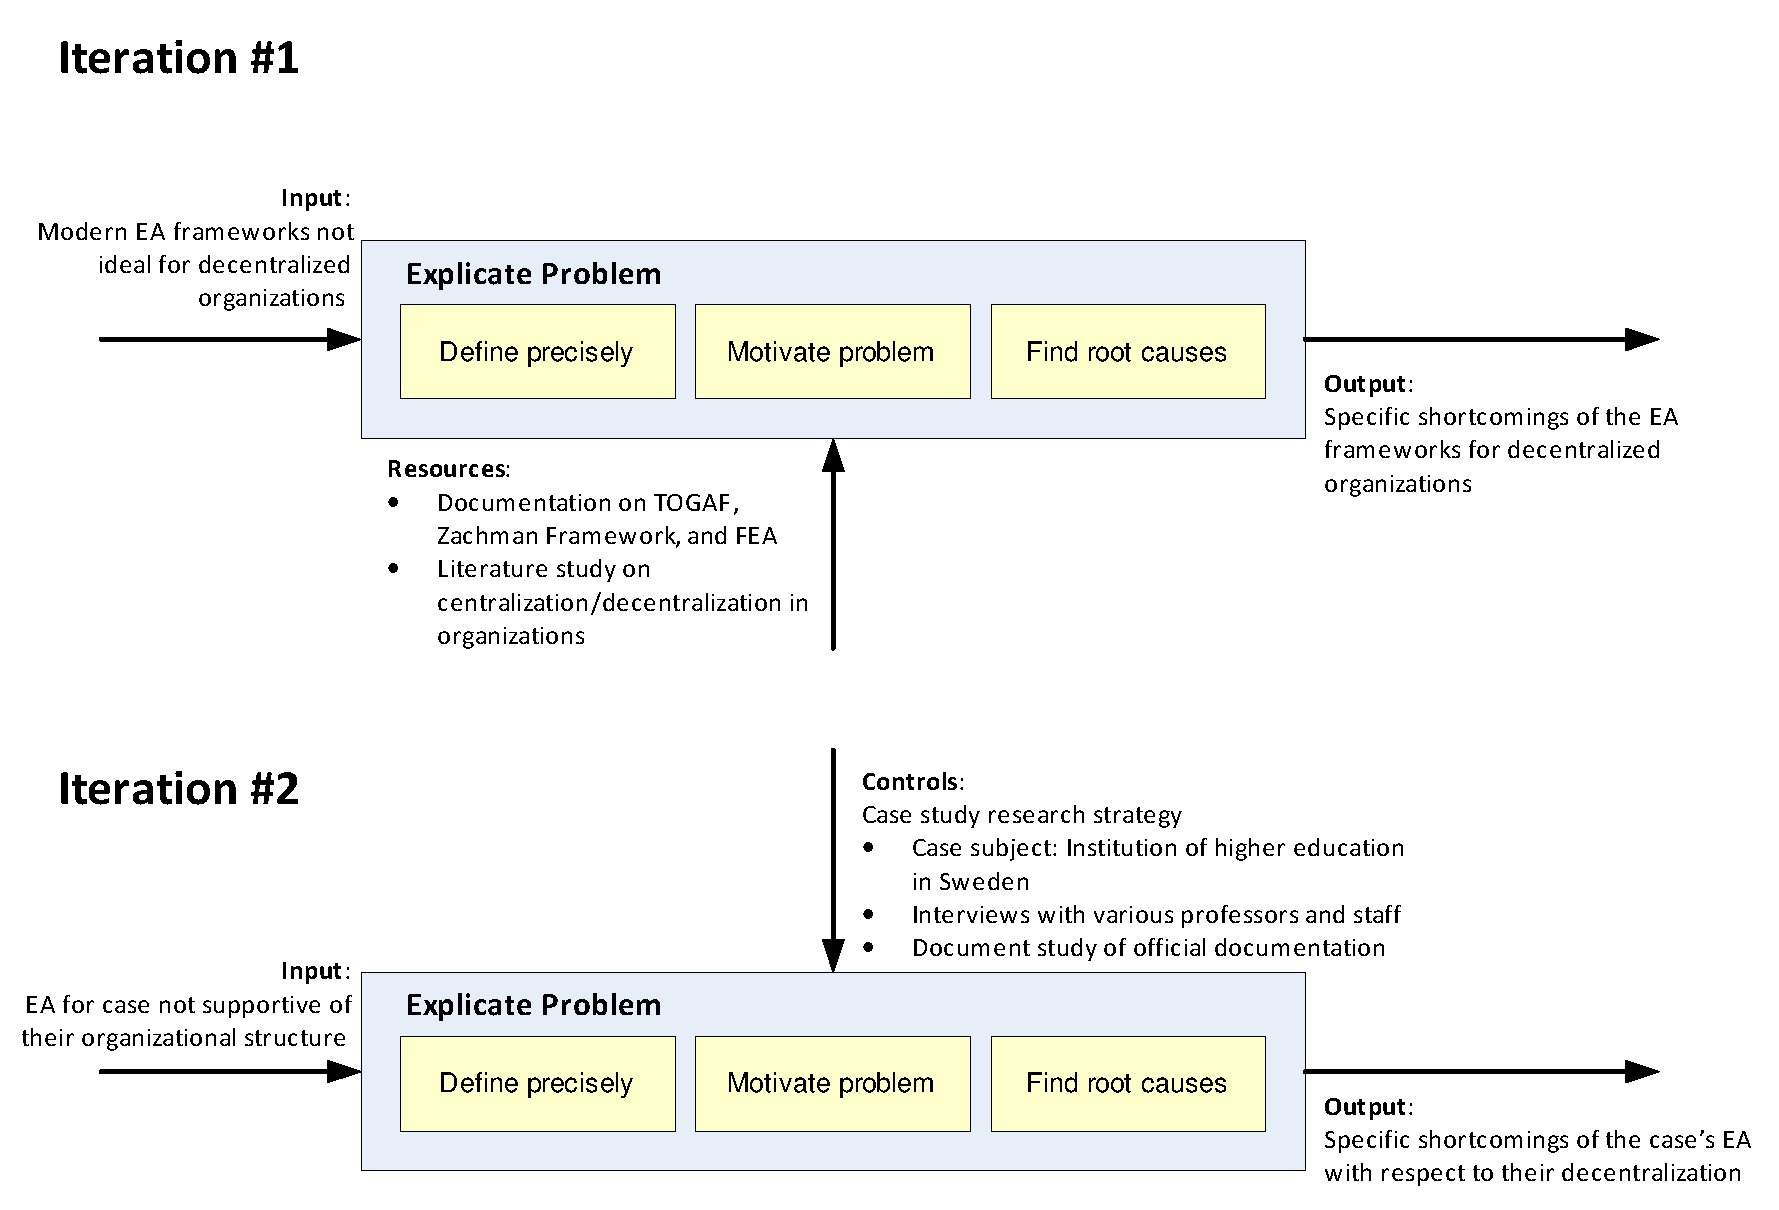
\includegraphics[scale=0.7]{method_problem}
\caption{Explicate problem activity}
\label{fig:method_problem}
\end{figure}

\subsubsection*{Outline artifact and define requirements}

Figure \ref{fig:method_outline} outlines the major components of this activity:
\begin{description}
  \item[Sub-activities] ``Outline artifact'' and ``define requirements''~\cite[Ch. 6]{johannessonPerjons2012}
  \item[Input] The fully explicated problem from the ``explicate problem'' activity
  \item[Resources] Literature study of organizational theory on decentralized organizations
  \item[Controls] None
  \item[Output] Requirements for a decentralized EA
\end{description}

In the first sub-activity ``outline artifact'', the type of artifacts being developed will be specified. 

In the second sub-activity, ``define requirements'', the requirements for the developed artifact will be elicited. This will be based on the fully explicated problem and the literature study on decentralized organizations.

\begin{figure}
\centering
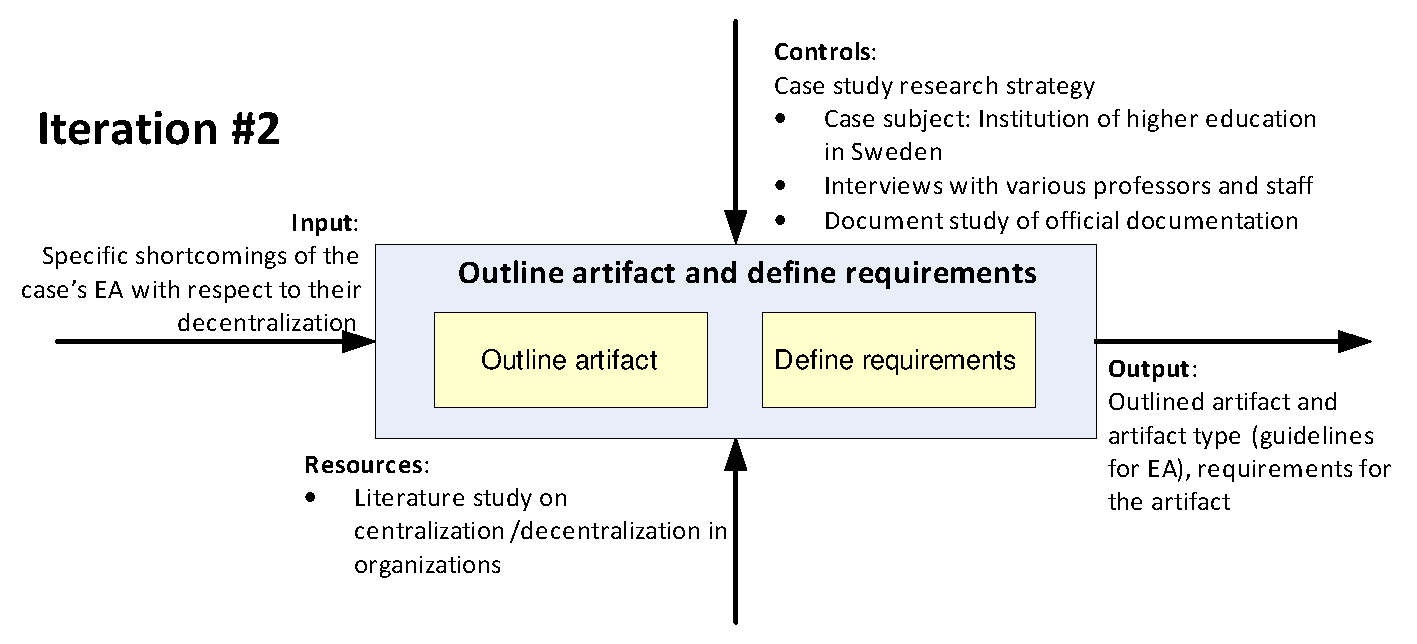
\includegraphics[scale=0.7]{method_outline}
\caption{Outline artifact and define requirements activity}
\label{fig:method_outline}
\end{figure}

\subsubsection*{Design and develop artifact}

Figure \ref{fig:method_design} outlines the major components of this activity:
\begin{description}
  \item[Sub-activities] ``Generate'' and ``search and select'' ~\cite[Ch. 7]{johannessonPerjons2012}
  \item[Input]  Requirements for a decentralized EA 
  \item[Resources] Literature study on peer-to-peer architectures
  \item[Controls] None
  \item[Output] Prototype of one artifact for one aspect of an EA framework for decentralized organizations 
\end{description}

In the ``generate'' sub-activity, different potential solutions, each covering a subset of the requirements from the ``outline artifact and define requirements activity'' will be outlined. This requires multiple artifacts as an EA framework is a large entity, composed of a number of different artifacts. In order to develop these artifacts, a literature study on peer-to-peer architectures has been conducted. Principles from peer-to-peer will be taken and applied as the basis for solutions meeting the specified requirements. Peer-to-peer architectures were chosen because they have offered solutions to decentralization in other domains (e.g. technical) and might therefore be able to provide solutions for the practice of EA. 

In the ``search and select'' sub-activity, one of the outlined solutions (from the ``generate'' sub-activity) will be selected and elaborated on to create a prototype of one artifact for an EA framework for decentralized organizations. 

\begin{figure}
\centering
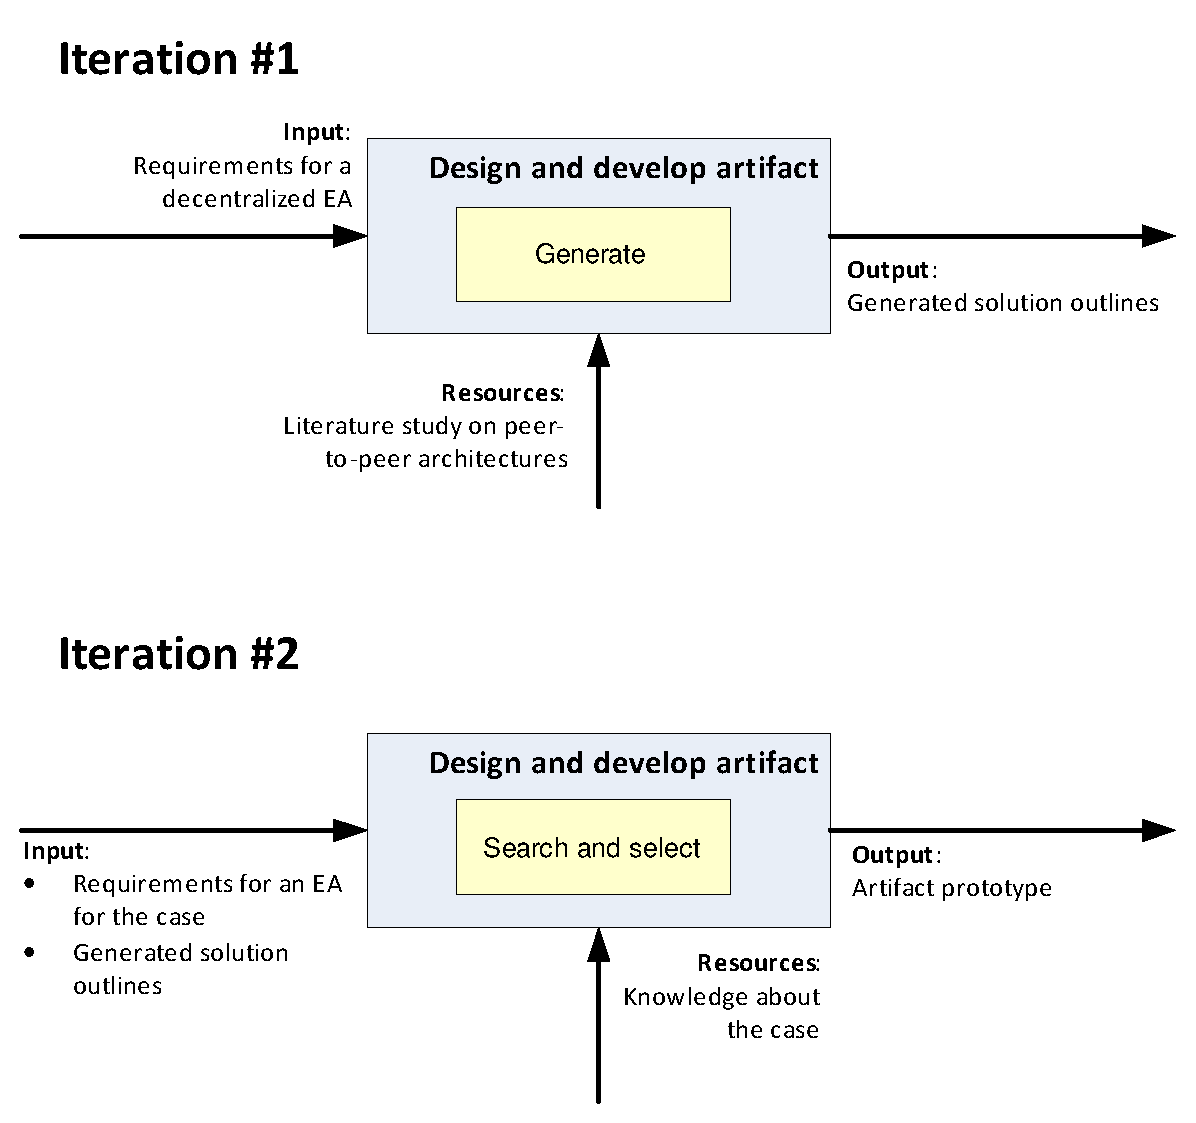
\includegraphics[scale=0.7]{method_design}
\caption{Design and develop artifact activity}
\label{fig:method_design}
\end{figure}
  
\subsubsection*{Demonstrate artifact}

Figure \ref{fig:method_demo} outlines the major components of this activity:
\begin{description}
  \item[Sub-activities]  ``Choose or design case'' and ``apply artifact''~\cite[Ch. 8]{johannessonPerjons2012}
  \item[Input]  Prototype of one artifact for one aspect of an EA framework for decentralized organizations
  \item[Resources]  Knowledge on the selected case (institution of higher education in Sweden)
  \item[Controls]  A case study research strategy that will make use of interviews and a document study
  \item[Output] Proof-of-concept artifact for one part of an EA framework prototype
\end{description}

For the ``choose or design case'', an institution of higher education in Sweden has been selected. Details on the case are described in \ref{sec:case}.

In the ``apply artifact'' sub-activity, the artifact will be applied to the case by creating a ``to-be'' architecture for the relevant aspect of the case. This ``to-be'' architecture will be the proof-of-concept artifact for one part of an EA framework prototype

\begin{figure}
\centering
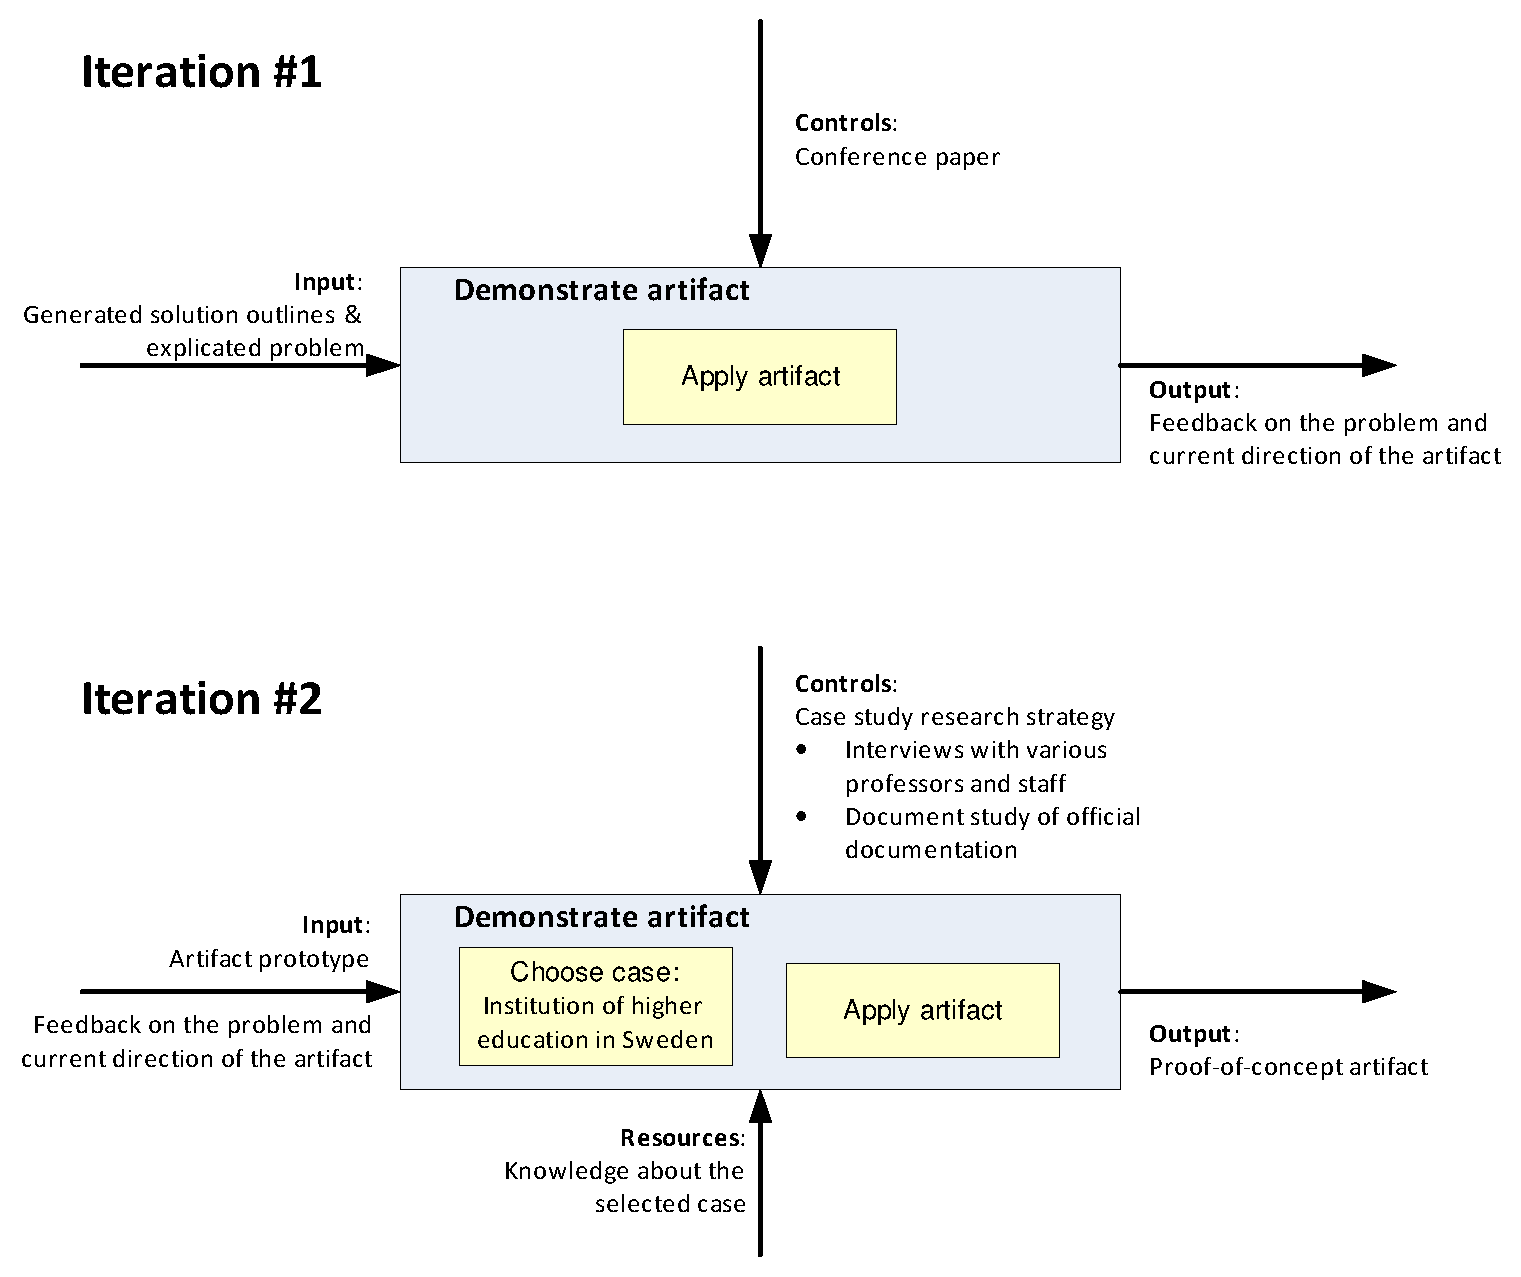
\includegraphics[scale=0.7]{method_demo}
\caption{Demonstrate artifact activity}
\label{fig:method_demo}
\end{figure}

\subsubsection*{Evaluate artifact}

The focus of this thesis work is on explicating the problem of decentralization for EA and demonstrating a proof-of-concept of a partial solution. Consequently, the evaluate artifact phase is not done. 

\section{Ethical Considerations}

As the proof-of-concept does not involve any actual implementation, the ethical considerations for this research project are minimal and only involve withholding the identity of the case institution. 

    
    %Part 3 - Results
    
    \chapter{Results}
    \label{chap:results}  
    
    \section{Explicate Problem}    
    \label{sec:problem}
    %\input{}


% Move to PROBLEM MOTIVATION
%Enterprise Architecture is a discipline  that allows an organization to construct and evolve its IT according to its needs. It provides a methodology and sets up a framework for assessing the current state of IT (architecture As-Is), for agreeing upon and communicating its future state (architecture To-Be), for planning, and for carrying out this transformation. Though, it is important that  EA methodology and structures acknowledge progressive decentralization and help the organization to tackle the challenges related to it.    
    
    
%    Thus, there is a need for better process management
%[17, 23] and for more integration within decentralized
%and modular individual enterprises (e.g. most discrete
%parts manufacturing companies) as well as among
%networks of enterprises belonging to the same group or
%cooperating on large collaborative projects (e.g.
%Daimler-Chrysler or the AIRBUS Consortium).
    
    \section{Outline Artifact and Define Requirements}
    \label{sec:outline}
    %\input{}    
    
    \section{Design and Develop Artifact}
    \label{sec:design}
    %\input{}
    
    \section{Demonstrate Artifact}
    \label{sec:demo}
    %\input{}    
    
    \chapter{Conclusion and Discussion}
    
    
    

    \backmatter
    % References
    % No restriction is set to the reference styles
    % Save your references in References.bib

    % \urlstyle{same}         
    % Uncomment the line above to make urls have the same font and
    % size as the surrounding text. 

%    from paper    
%    \renewcommand{\baselinestretch}{0.98}
%    \bibliographystyle{IEEEtran}
%    {\small
%    \bibliography{biblioDecentralizedEA}
%    }
%    \renewcommand{\baselinestretch}{1}

%    from SU
%    \bibliographystyle{plain}
%    \bibliography{biblioDecentralizedEA}


    \bibliographystyle{IEEEtran}
    \bibliography{biblioDecentralizedEA}

%    \finalpageDSV

\end{document}